\chapter{Introduction}
\label{cha:Introduction}

%\begin{figure}
%    \centering
%    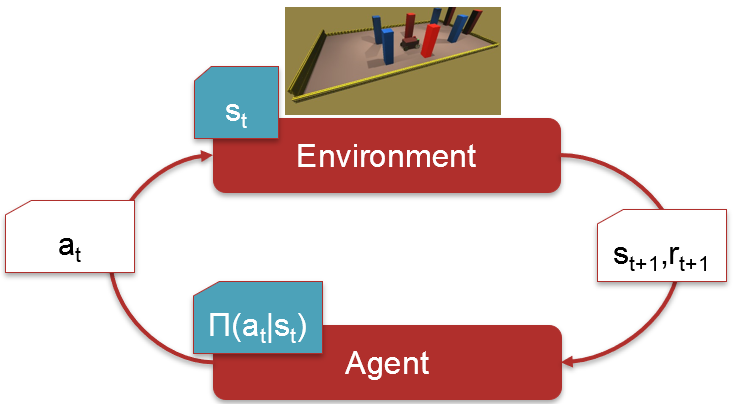
\includegraphics[width=0.8\textwidth]{Bilder/rl_cycle.png}
%    \caption{Loop in Collect Data}
%    \label{fig:unitycommunication}
%\end{figure} % TODO can we use this image?

Recent avancements in artificial intelligence technology have made it possible to develop automated solutons for a wide range of tasks that were previously thought to be too complex and unfit for machines to solve. Most notably over the last few years is the introduction of diffusion image models and large language models. These technologies were well recieved and moved artificial intelligence tools into public discourse. All over the world people have recognized the potential of artificial intelligence technologies and are now using them in their daily life and at work.

Artificial intelligence has already been of big importance in academia and industry for a long time. AI has been proved useful in many different fields, such as image recognition, natural language processing, and robotics. This encourages researchers and industry to further develop and use AI in their work. A promissing domain for the application of AI is autonomous driving.

The development of autonomous vehicles promises to greatly reduce the number of traffic accidents and transportation cost \textcite{mckinsey}. The development of autonomous driving could have further downstream effects on our society and industry, such as for example improved logistic and transportation systems.
As a result, researchers and private enterprises from all over the globe are making progress towards fully autonomous driving agents. Many companies started to integrate adaptive cruise control and lane centering assistance \textcite{carreviews} in their products. Due to the recent developments in artificial intelligence and the very high complexity of the task of autonomous driving, artificial intelligence often plays a big role in these systems \textcite{drl_for_ad}.

Predictions for the future of autonomous driving have been very optimistic and although huge progress has been made, the task of fully autonomous driving is still far from being solved \textcite{state_of_autonomous_driving2023}. This thesis aims at contributing to the research in this field by applying reinforcement learning to autonomous driving agents in a simulated environment. This work builds upon the work of \textcite{maximilian} and will use the same task and evaluation metrics. This thesis focusses on improving the agent's resiliency to changing light conditions by training a convolutional neural network end-to-end using reinforcement learning.
